\documentclass{beamer}

\usepackage{tikz}
\usepackage{xstring}
\usepackage{amsmath}
\usetikzlibrary{calc}


\title{Starter}
\date{}

\newcommand{\cuboid}[4]{
\begin{scope}[shift={(#1,#2)}]
  % Draw the cuboid
  \draw (0,0) rectangle (2,1);
  \draw (0.6,0.6) rectangle (2.6,1.6);
  \draw (0,0) -- (0.6,0.6);
  \draw (2,0) -- (2.6,0.6);
  \draw (2,1) -- (2.6,1.6);
  \draw (0,1) -- (0.6,1.6);

  % Labels (letter above, dimensions below)
  \node at (1,-0.4) {\tiny \bf{#3}};
  \node at (1,-1.2) {\tiny #4};

  % ----- Parse dimension string #4 (format: width×height×depth) -----
  \StrBefore{#4}{×}[\widthstr]                % first number
  \StrBehind{#4}{×}[\temp]                    % rest = height×depth
  \StrBefore{\temp}{×}[\heightstr]             % second number
  \StrBehind{\temp}{×}[\depthstr]               % third number

  % ----- Width dimension (bottom front edge) -----
  \draw (0,0) -- (0,-0.6);                     % left extension
  \draw (2,0) -- (2,-0.6);                      % right extension
  \draw (0,-0.8) -- (2,-0.8);                   % dimension line
  % ticks at ends (vertical)
  \draw (0,-0.75) -- (0,-0.85);
  \draw (2,-0.75) -- (2,-0.85);
  % label
  \node at (1,-0.8) [fill=white, inner sep=1pt] {\tiny \widthstr};

  % ----- Height dimension (left front edge) -----
  \draw (0,0) -- (-0.6,0);                      % lower extension
  \draw (0,1) -- (-0.6,1);                       % upper extension
  \draw (-0.8,0) -- (-0.8,1);                    % dimension line
  % ticks at ends (horizontal)
  \draw (-0.75,0) -- (-0.85,0);
  \draw (-0.75,1) -- (-0.85,1);
  % label
  \node at (-0.8,0.5) [fill=white, inner sep=1pt] {\tiny \heightstr};

    % ----- Depth dimension (bottom right edge) -----
    \coordinate (B) at (2,0);
    \coordinate (F) at (2.6,0.6);
    \coordinate (dir) at ($(F)-(B)$);              % direction of edge (0.6,0.6)
    % outward offset perpendicular to edge (along (1,-1) direction)
    \coordinate (offset) at (0.3,-0.3);
    % shorten factor: move endpoints inward along dir
    \def\shorten{0.1}
    \coordinate (start) at ($(B)+(offset)+\shorten*(dir)$);
    \coordinate (end)   at ($(F)+(offset)-\shorten*(dir)$);
    % dimension line
    \draw (start) -- (end);
    % ticks perpendicular to dimension line (along direction of edge)
    \coordinate (tickDir) at ($(0,0)!0.1!(dir)$);        % vector for tick length
\coordinate (start) at ($(B)+(offset)+(0,0)!\shorten!(dir)$);
\coordinate (end)   at ($(F)+(offset)-(0,0)!\shorten!(dir)$);;
    % label
    \node at ($(start)!0.5!(end)$) [fill=white, inner sep=1pt] {\tiny \depthstr};
\end{scope}
}

\begin{document}

%------------------------------------------------
% QUESTIONS SLIDE
%------------------------------------------------

\begin{frame}

\begin{columns}[T]

% LEFT COLUMN
\column{0.5\textwidth}

\textbf{1.}

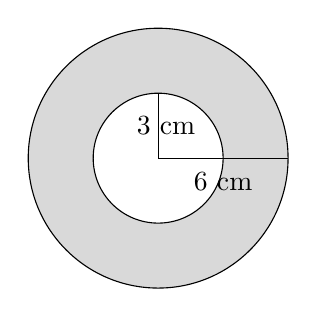
\begin{tikzpicture}[scale=0.55]
\def\R{3}
\def\r{1.5}

\fill[gray!30] (0,0) circle (\R);
\fill[white] (0,0) circle (\r);

\draw (0,0) circle (\R);
\draw (0,0) circle (\r);

\draw (0,0) -- (\R,0);
\draw (0,0) -- (0,\r);

% FIXED: Use separate coordinates for midpoint calculation
\path (0,0) -- (\R,0) coordinate[midway] (midR);
\path (0,0) -- (0,\r) coordinate[midway] (midr);
\node at (midR) [yshift=-0.3cm] {$6$ cm};
\node at (midr) [xshift=+0.1cm] {$3$ cm};
\end{tikzpicture}

\vspace{0.2cm}
Find the shaded area.

\vspace{0.4cm}

\textbf{3.}

\begin{tikzpicture}[scale=0.45]

\draw (0,0) rectangle (3,2);
\node at (1.5,-0.4) {\small A};
\node at (1.5,2.5) {6};
\node at (-0.4,1) {4};

\draw (5,0) rectangle (9.5,3);
\node at (7.25,-0.4) {\small B};
\node at (7.25,3.5) {9};
\node at (4.6,1.5) {6};

\end{tikzpicture}

Find the scale factor mapping \newline A → B.

% RIGHT COLUMN
\column{0.5\textwidth}

\textbf{2.}

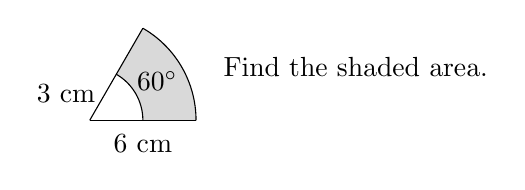
\begin{tikzpicture}[scale=0.45]
\def\R{3}
\def\r{1.5}
\def\angle{60}

% Shaded annular sector
\fill[gray!30] (0,0) -- (0:\R) arc (0:\angle:\R) -- cycle;
\fill[white] (0,0) -- (0:\r) arc (0:\angle:\r) -- cycle;

% Draw only the arcs that bound the shaded region (no full circles)
\draw (0:\R) arc (0:\angle:\R);
\draw (0:\r) arc (0:\angle:\r);

% Draw the two radii
\draw (0,0) -- (0:\R);
\draw (0,0) -- (\angle:\R);

% Labels
\node at ($(0,0)!0.5!(\R,0)$) [yshift=-0.3cm] {$6$ cm};
\node at ($(0,0)!0.5!(0,\r)$) [xshift=-0.3cm] {$3$ cm};
\node at (\angle/2:2.2) {$60^\circ$};

% Add question text to the right of the diagram
\node[anchor=west] at (3.5,1.5) {\text{Find the shaded area.}};
\end{tikzpicture}


\textbf{4.}
\begin{center}
 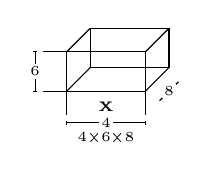
\begin{tikzpicture}[scale=0.5]
    \cuboid{0}{0}{X}{4×6×8}
\end{tikzpicture}
\end{center}

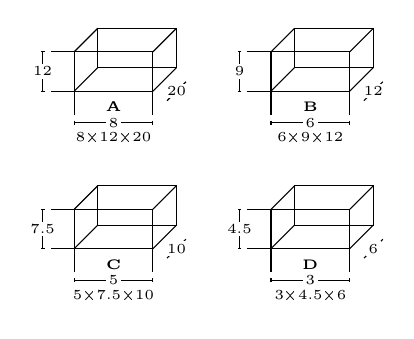
\begin{tikzpicture}[scale=0.5]
  \cuboid{0}{-2}{A}{8×12×20}
  \cuboid{5}{-2}{B}{6×9×12}
  \cuboid{0}{-6}{C}{5×7.5×10}
  \cuboid{5}{-6}{D}{3×4.5×6}
\end{tikzpicture}

Which are similar to $X$?

\end{columns}

\end{frame}

%------------------------------------------------
% ANSWERS SLIDE
%------------------------------------------------

\begin{frame}

\begin{columns}[T]

% LEFT COLUMN
\column{0.5\textwidth}

\textbf{1.}

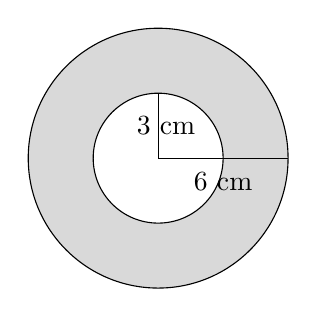
\begin{tikzpicture}[scale=0.55]
\def\R{3}
\def\r{1.5}

\fill[gray!30] (0,0) circle (\R);
\fill[white] (0,0) circle (\r);

\draw (0,0) circle (\R);
\draw (0,0) circle (\r);

\draw (0,0) -- (\R,0);
\draw (0,0) -- (0,\r);

% FIXED: Use separate coordinates for midpoint calculation
\path (0,0) -- (\R,0) coordinate[midway] (midR);
\path (0,0) -- (0,\r) coordinate[midway] (midr);
\node at (midR) [yshift=-0.3cm] {$6$ cm};
\node at (midr) [xshift=0.1cm] {$3$ cm};
\end{tikzpicture}

{\color{red} \(\pi6^2 - \pi3^2 = 27\pi\ \text{cm}^2\)}

\vspace{0.4cm}

\textbf{3.}

\begin{tikzpicture}[scale=0.45]

\draw (0,0) rectangle (3,2);
\node at (1.5,-0.4) {\small A};
\node at (1.5,2.5) {6};
\node at (-0.4,1) {4};

\draw (5,0) rectangle (9.5,3);
\node at (7.25,-0.4) {\small B};
\node at (7.25,3.5) {9};
\node at (4.6,1.5) {6};

\end{tikzpicture}

{\color{red} Scale factor = \(1.5\)}

% RIGHT COLUMN
\column{0.5\textwidth}

\textbf{2.}

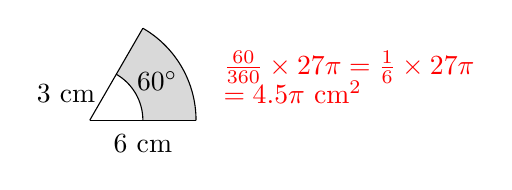
\begin{tikzpicture}[scale=0.45]
\def\R{3}
\def\r{1.5}
\def\angle{60}

% Shaded annular sector
\fill[gray!30] (0,0) -- (0:\R) arc (0:\angle:\R) -- cycle;
\fill[white] (0,0) -- (0:\r) arc (0:\angle:\r) -- cycle;

% Draw only the arcs that bound the shaded region (no full circles)
\draw (0:\R) arc (0:\angle:\R);
\draw (0:\r) arc (0:\angle:\r);

% Draw the two radii
\draw (0,0) -- (0:\R);
\draw (0,0) -- (\angle:\R);

% Labels
\node at ($(0,0)!0.5!(\R,0)$) [yshift=-0.3cm] {$6$ cm};
\node at ($(0,0)!0.5!(0,\r)$) [xshift=-0.3cm] {$3$ cm};
\node at (\angle/2:2.2) {$60^\circ$};

% Add answer text to the right of the diagram
\node[anchor=west] at (3.5,1.5) {\color{red} \(\frac{60}{360} \times 27\pi = \frac{1}{6}\times27\pi\)};
\node[anchor=west] at (3.5,0.8) {\color{red} \(= 4.5\pi\ \text{cm}^2\)};
\end{tikzpicture}

\vspace{0.2cm}

\textbf{4.}

\begin{center}
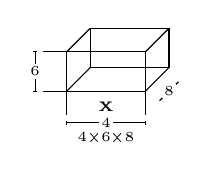
\begin{tikzpicture}[scale=0.5]
    \cuboid{0}{0}{X}{4×6×8}
\end{tikzpicture}
\end{center}

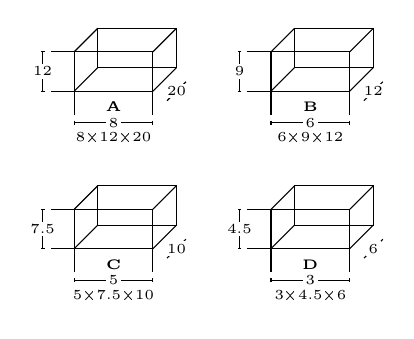
\begin{tikzpicture}[scale=0.5]
  \cuboid{0}{-2}{A}{8×12×20}
  \cuboid{5}{-2}{B}{6×9×12}
  \cuboid{0}{-6}{C}{5×7.5×10}
  \cuboid{5}{-6}{D}{3×4.5×6}
\end{tikzpicture}

{\color{red} Similar shapes: B, C, D}  % Corrected based on proportions

\end{columns}

\end{frame}

\end{document}